\section{Rezultati testiranja}
Rezultati testiranja podjeljeni su prema stranicama koje predstavljaju određeni tip web sadržaja:

\begin{enumerate}
    \item \hyperref[sec:rezultati-o-nama]{\textbf{Stranica O nama}} - statični sadržaj
    \item \hyperref[sec:rezultati-blog]{\textbf{Stranica Blog}} - dinamički sadržaj s listom blog postova
    \item \hyperref[sec:rezultati-blog-post]{\textbf{Stranica pojedinog blog posta}} - dinamički sadržaj s detaljima pojedinog blog posta
\end{enumerate}

\bigskip
\noindent
Za prikaz rezultata pojedine stranice odabrani su slijedeći grafovi i tablice:

\begin{itemize}
    \item \textbf{Ukupna ocjena radnih značajki programskog okvira}
    \item \textbf{Ukupna ocjena radnih značajki programskog okvira po metrici}
    \item \textbf{Ocjene kombinacije programskog okvira i strategije iscrtavanja po metrici (postotak)}
    \item \textbf{Ocjene kombinacije programskog okvira i strategije iscrtavanja po metrici (vrijednosti)}
    \item \textbf{Ocjene strategije iscrtavanja po programskom okviru}
    \item \textbf{Sažetak rezultata po kategorijama} - tablica
\end{itemize}

\bigskip
\noindent
Ukupni rezultati cijelokupne aplikacije:

\begin{itemize}
    \item \hyperref[fig:ukupne_ocjene_radnih_znacajki]{\textbf{Ukupne ocjene radnih značajki programskih okvira po tipu stranice}}
    \item \hyperref[fig:ukupne_ocjene_strategija_iscrtavanja]{\textbf{Ocjene strategija iscrtavanja po tipu stranice}}
    \item \hyperref[tab:usporedba_metrika_po_tipu_stranice]{\textbf{Usporedba metrika po tipu stranice}} - tablica
\end{itemize}

\bigskip
\noindent
Za prikaz dodatnih metrika odabrani su slijedeći grafovi i tablice:

\begin{itemize}
    \item \hyperref[fig:average_build_times_by_framework_and_strategy]{\textbf{Srednje vrijednosti vremena izgradnje po strategiji iscrtavanja}}
    \item \hyperref[fig:average_bundle_size_by_strategy]{\textbf{Srednja veličina JS paketa po strategiji iscrtavanja}}
    \item \hyperref[fig:average_scripting_performance_times]{\textbf{Srednja vremena skriptiranja po strategiji iscrtavanja}}
    \item \hyperref[fig:build_times_heat_map]{\textbf{Mapa topline vremena izgradnje po strategiji iscrtavanja}}
    \item \hyperref[fig:bundle_size_distribution_by_framework]{\textbf{Raspodjela veličine JS paketa po programskom okviru}}
    \item \hyperref[fig:bundle_size_vs_build_time_correlation]{\textbf{Odnos između veličine JS paketa i vremena izgradnje}}
    \item \hyperref[fig:overall_framework_build_performance]{\textbf{Srednja vrijednost vremena izgradnje po programskom okviru}}
    \item \hyperref[fig:performance_vs_bundle_size_tradeoff]{\textbf{Kompromis između vremena skriptiranja i veličine JS paketa}}
\end{itemize}

\subsection{Rezultati testiranja stranice O nama}
\label{sec:rezultati-o-nama}

\begin{figure}[H]
    \centering
    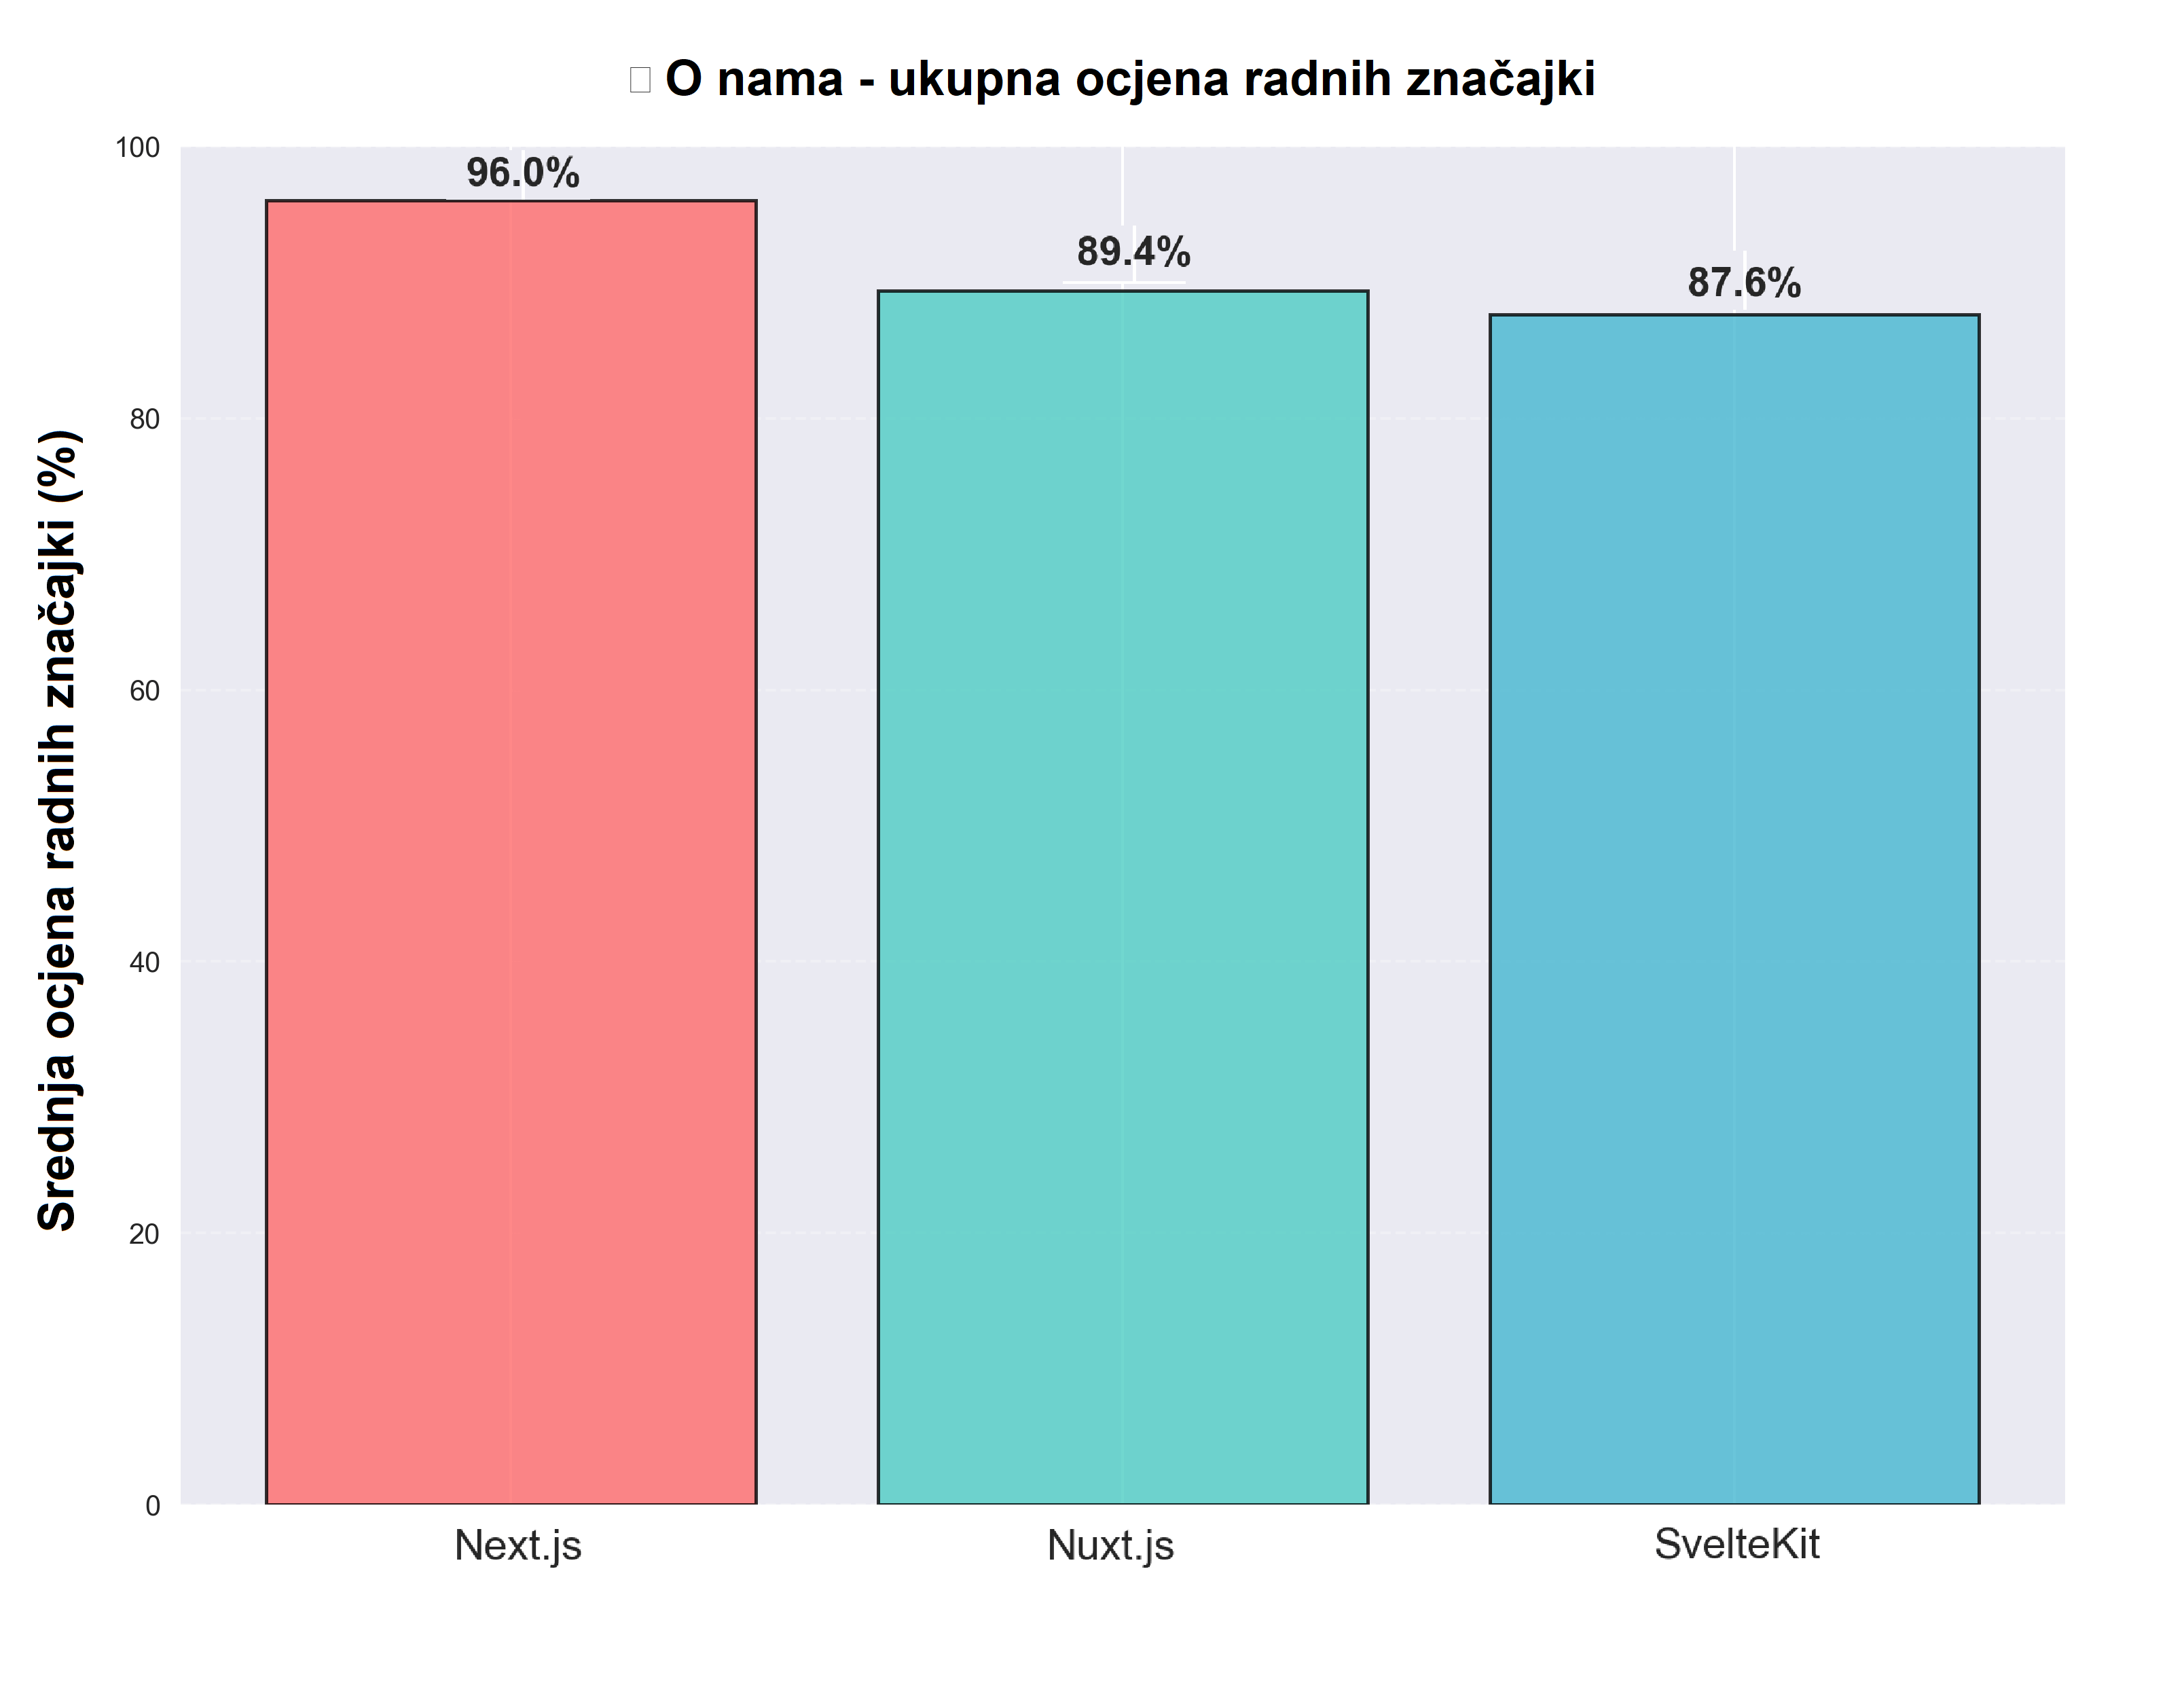
\includegraphics[width=0.8\textwidth]{slike/rezultati/about/about_framework_overall_performance.png}
    \caption{Ukupna ocjena radnih značajki programskih okvira (stranica O nama)}
    \label{fig:testiranje-o-nama-ukupne-performanse}
\end{figure}

\begin{figure}[H]
    \centering
    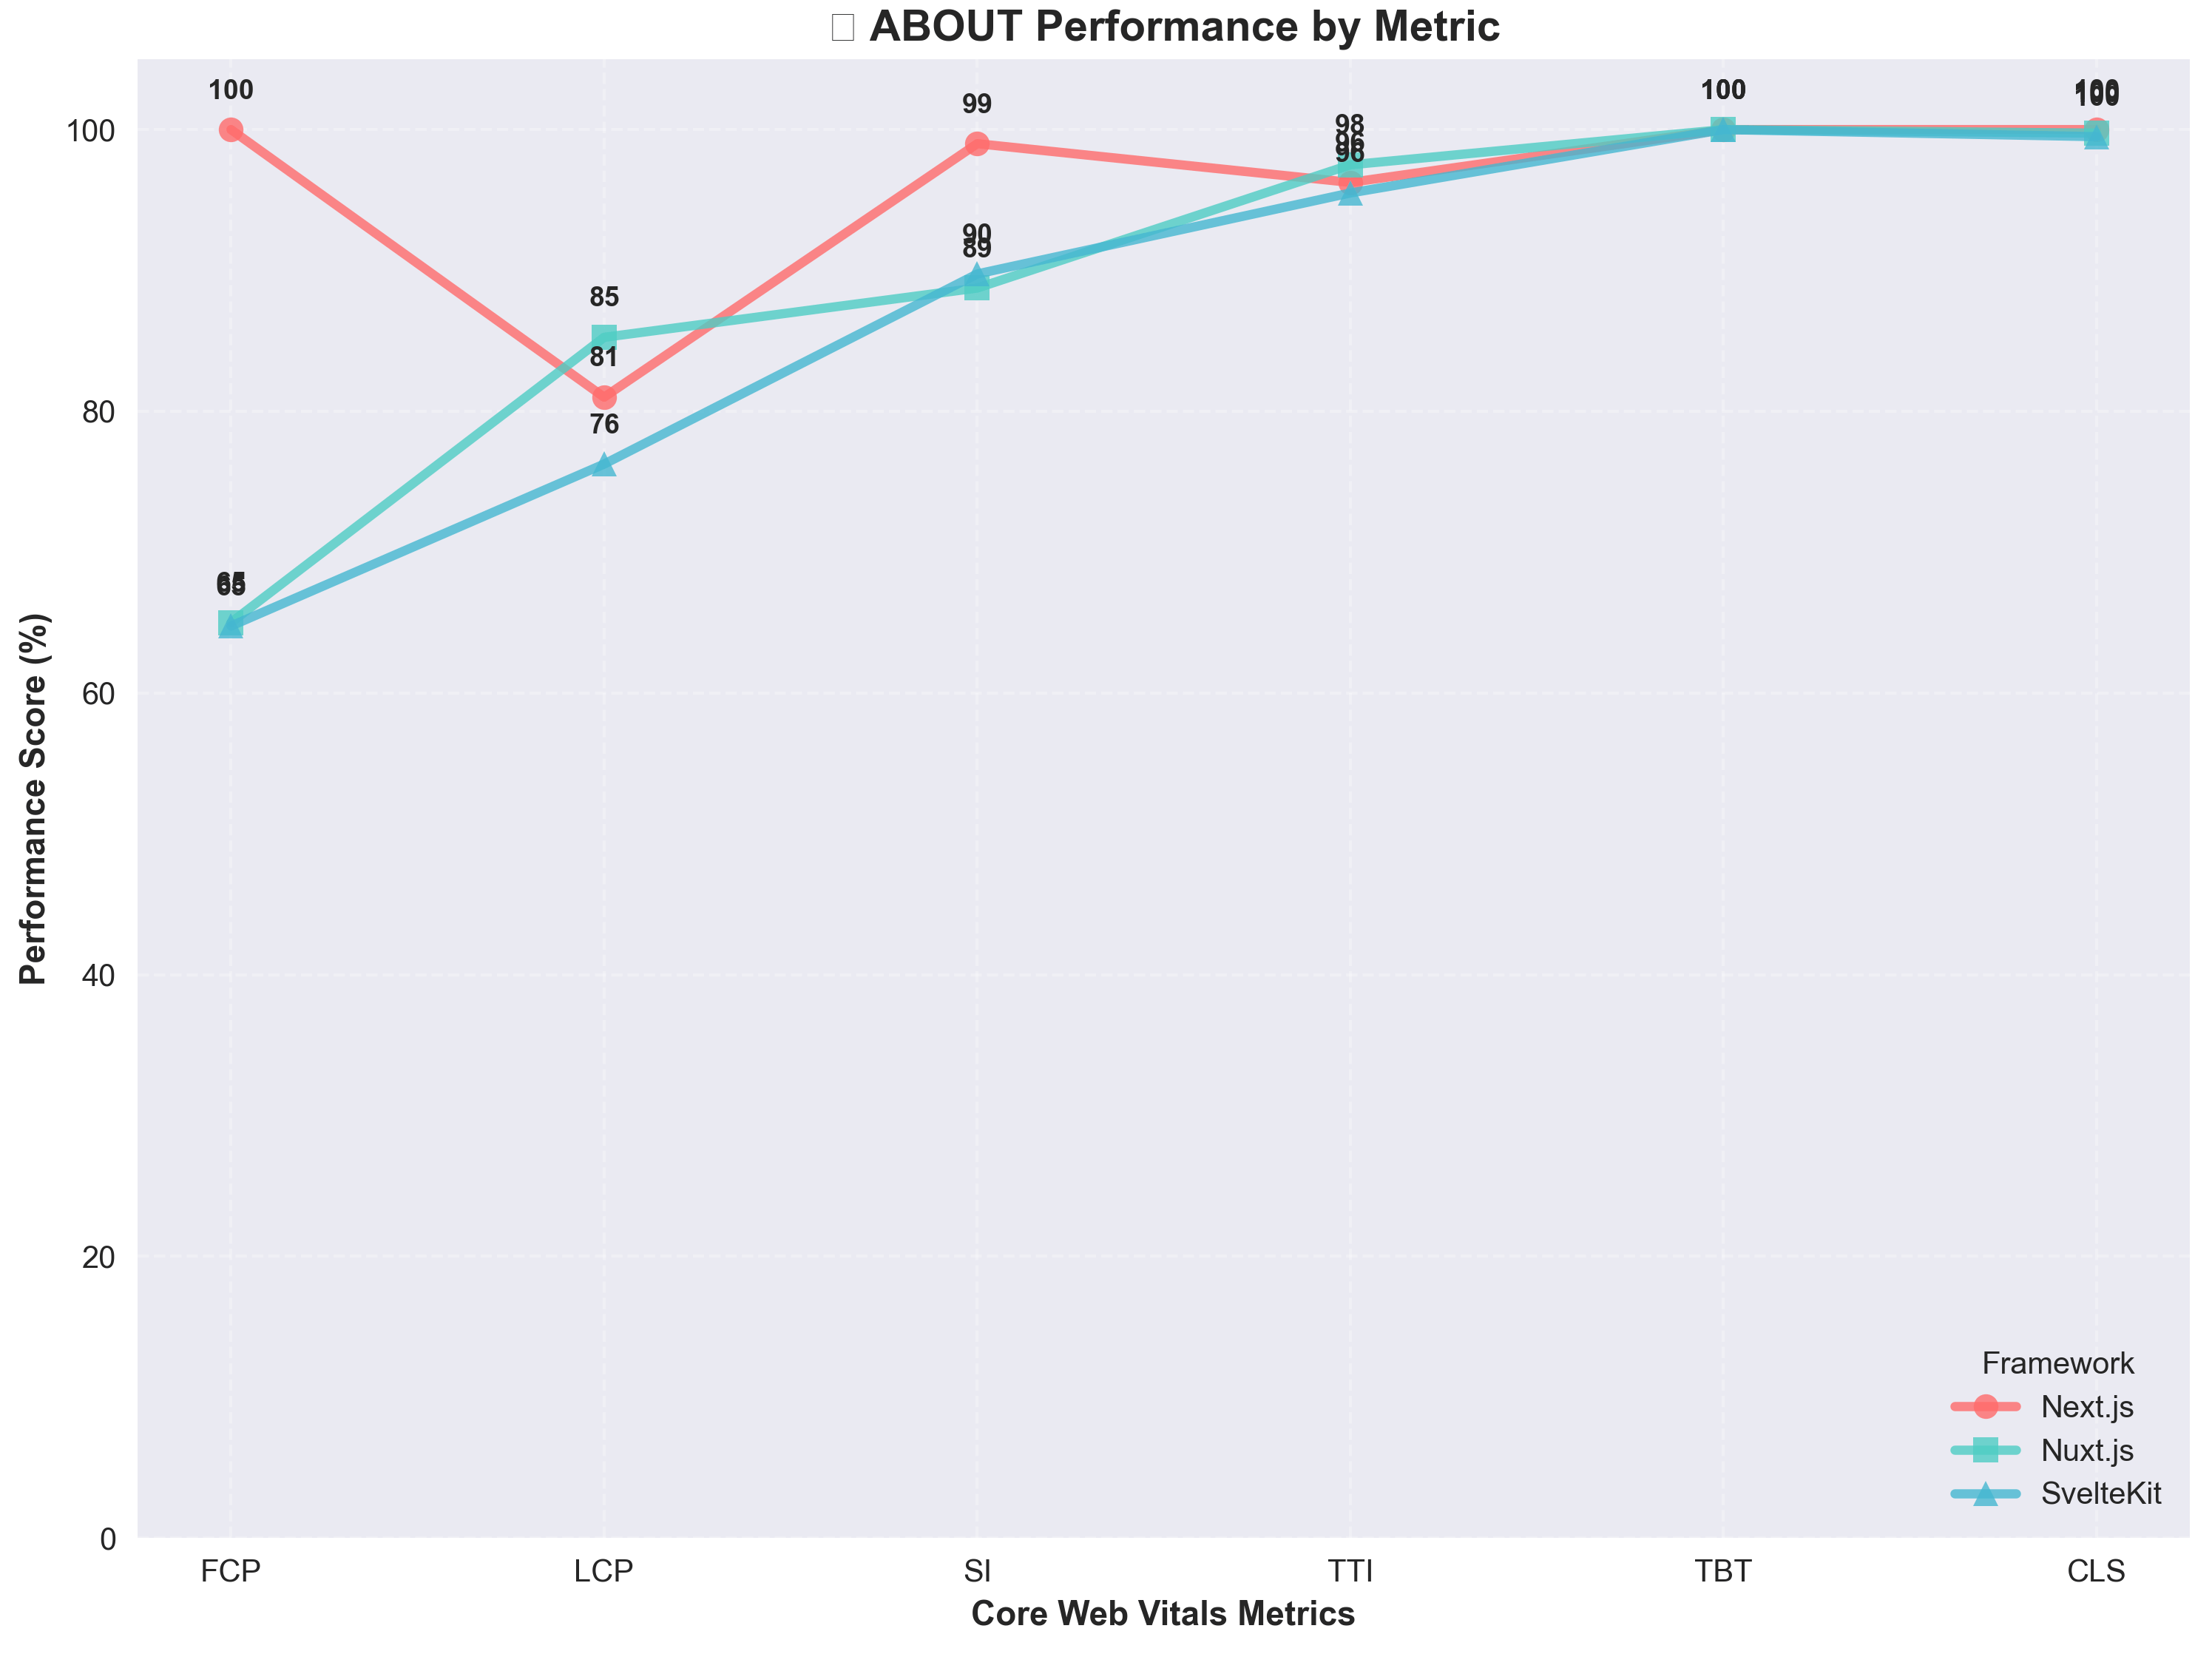
\includegraphics[width=0.8\textwidth]{slike/rezultati/about/about_performance_by_metric.png}
    \caption{Ukupna ocjena radnih značajki programskih okvira po metrici (stranica O nama)}
    \label{fig:testiranje-o-nama-performanse-po-metrici}
\end{figure}

\begin{figure}[H]
    \centering
    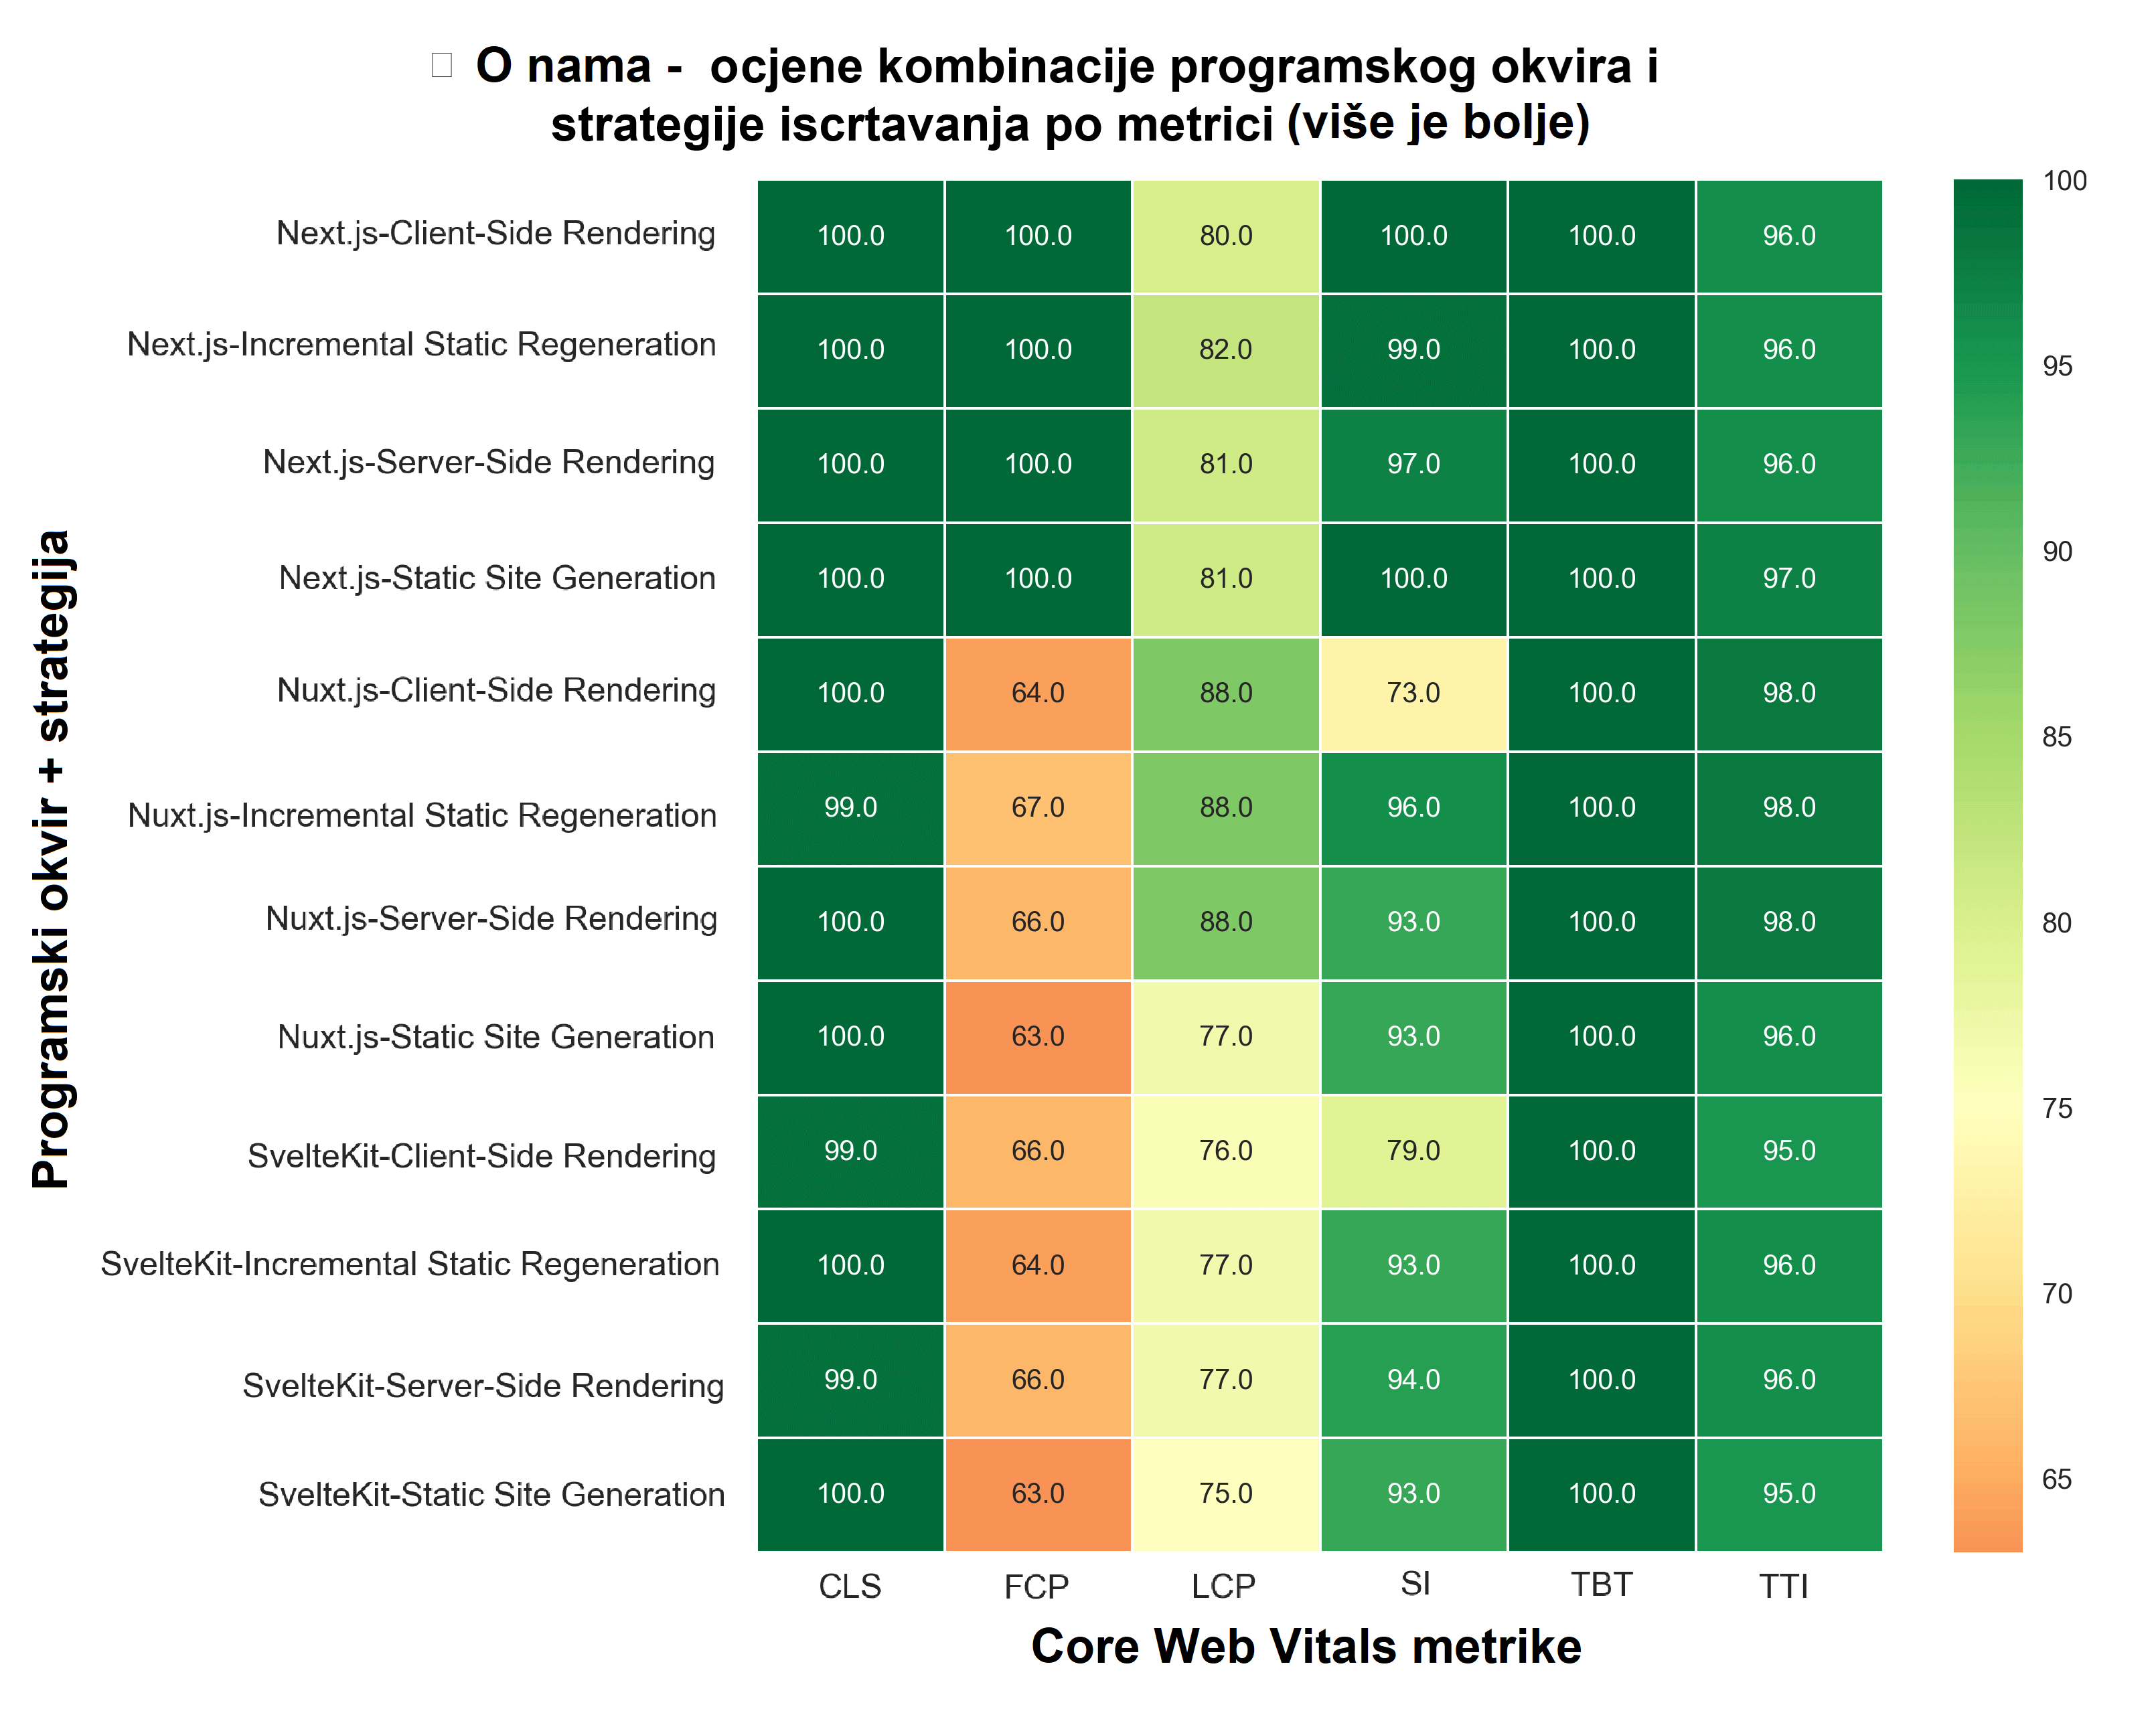
\includegraphics[width=\textwidth]{slike/rezultati/about/about_performance_scores.png}
    \caption{Ocjene kombinacije programskog okvira i strategije iscrtavanja po metrici - postotak (stranica O nama)}
    \label{fig:testiranje-o-nama-postotak}
\end{figure}

\begin{figure}[H]
    \centering
    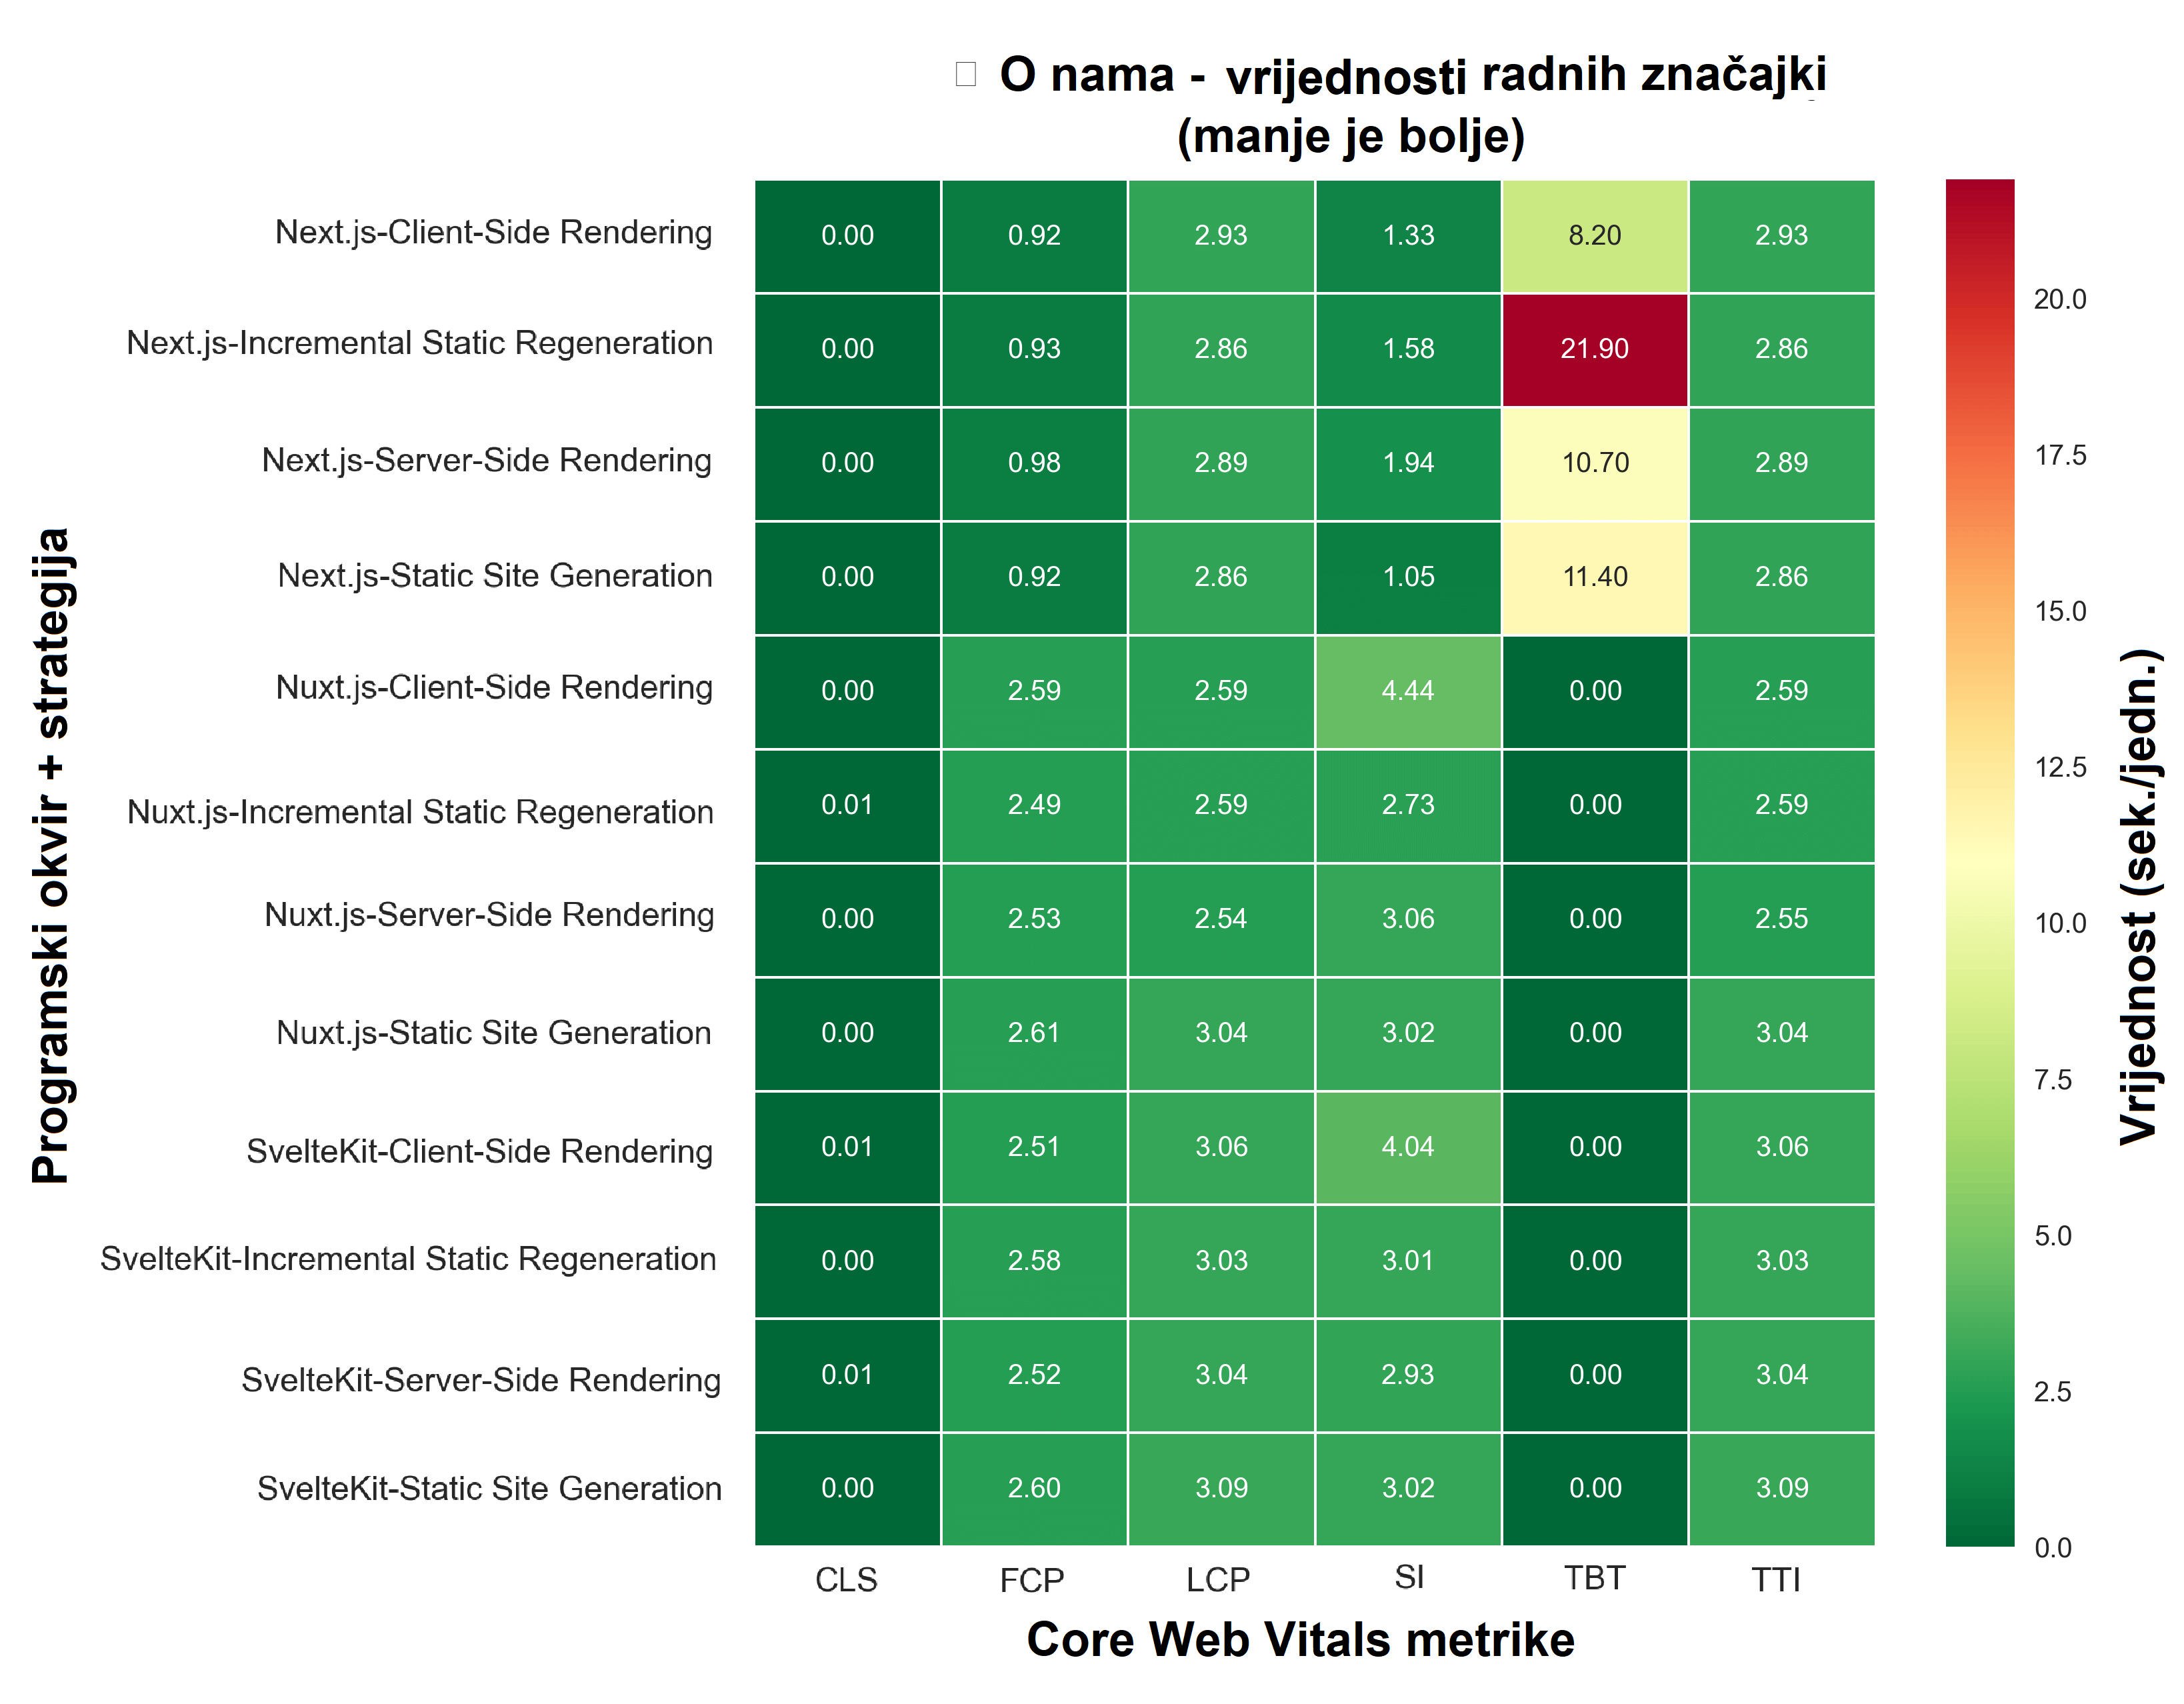
\includegraphics[width=\textwidth]{slike/rezultati/about/about_performance_values.png}
    \caption{Ocjene kombinacije programskog okvira i strategije iscrtavanja po metrici - vrijednosti (stranica O nama)}
    \label{fig:testiranje-o-nama-vrijednosti}
\end{figure}

\begin{figure}[H]
    \centering
    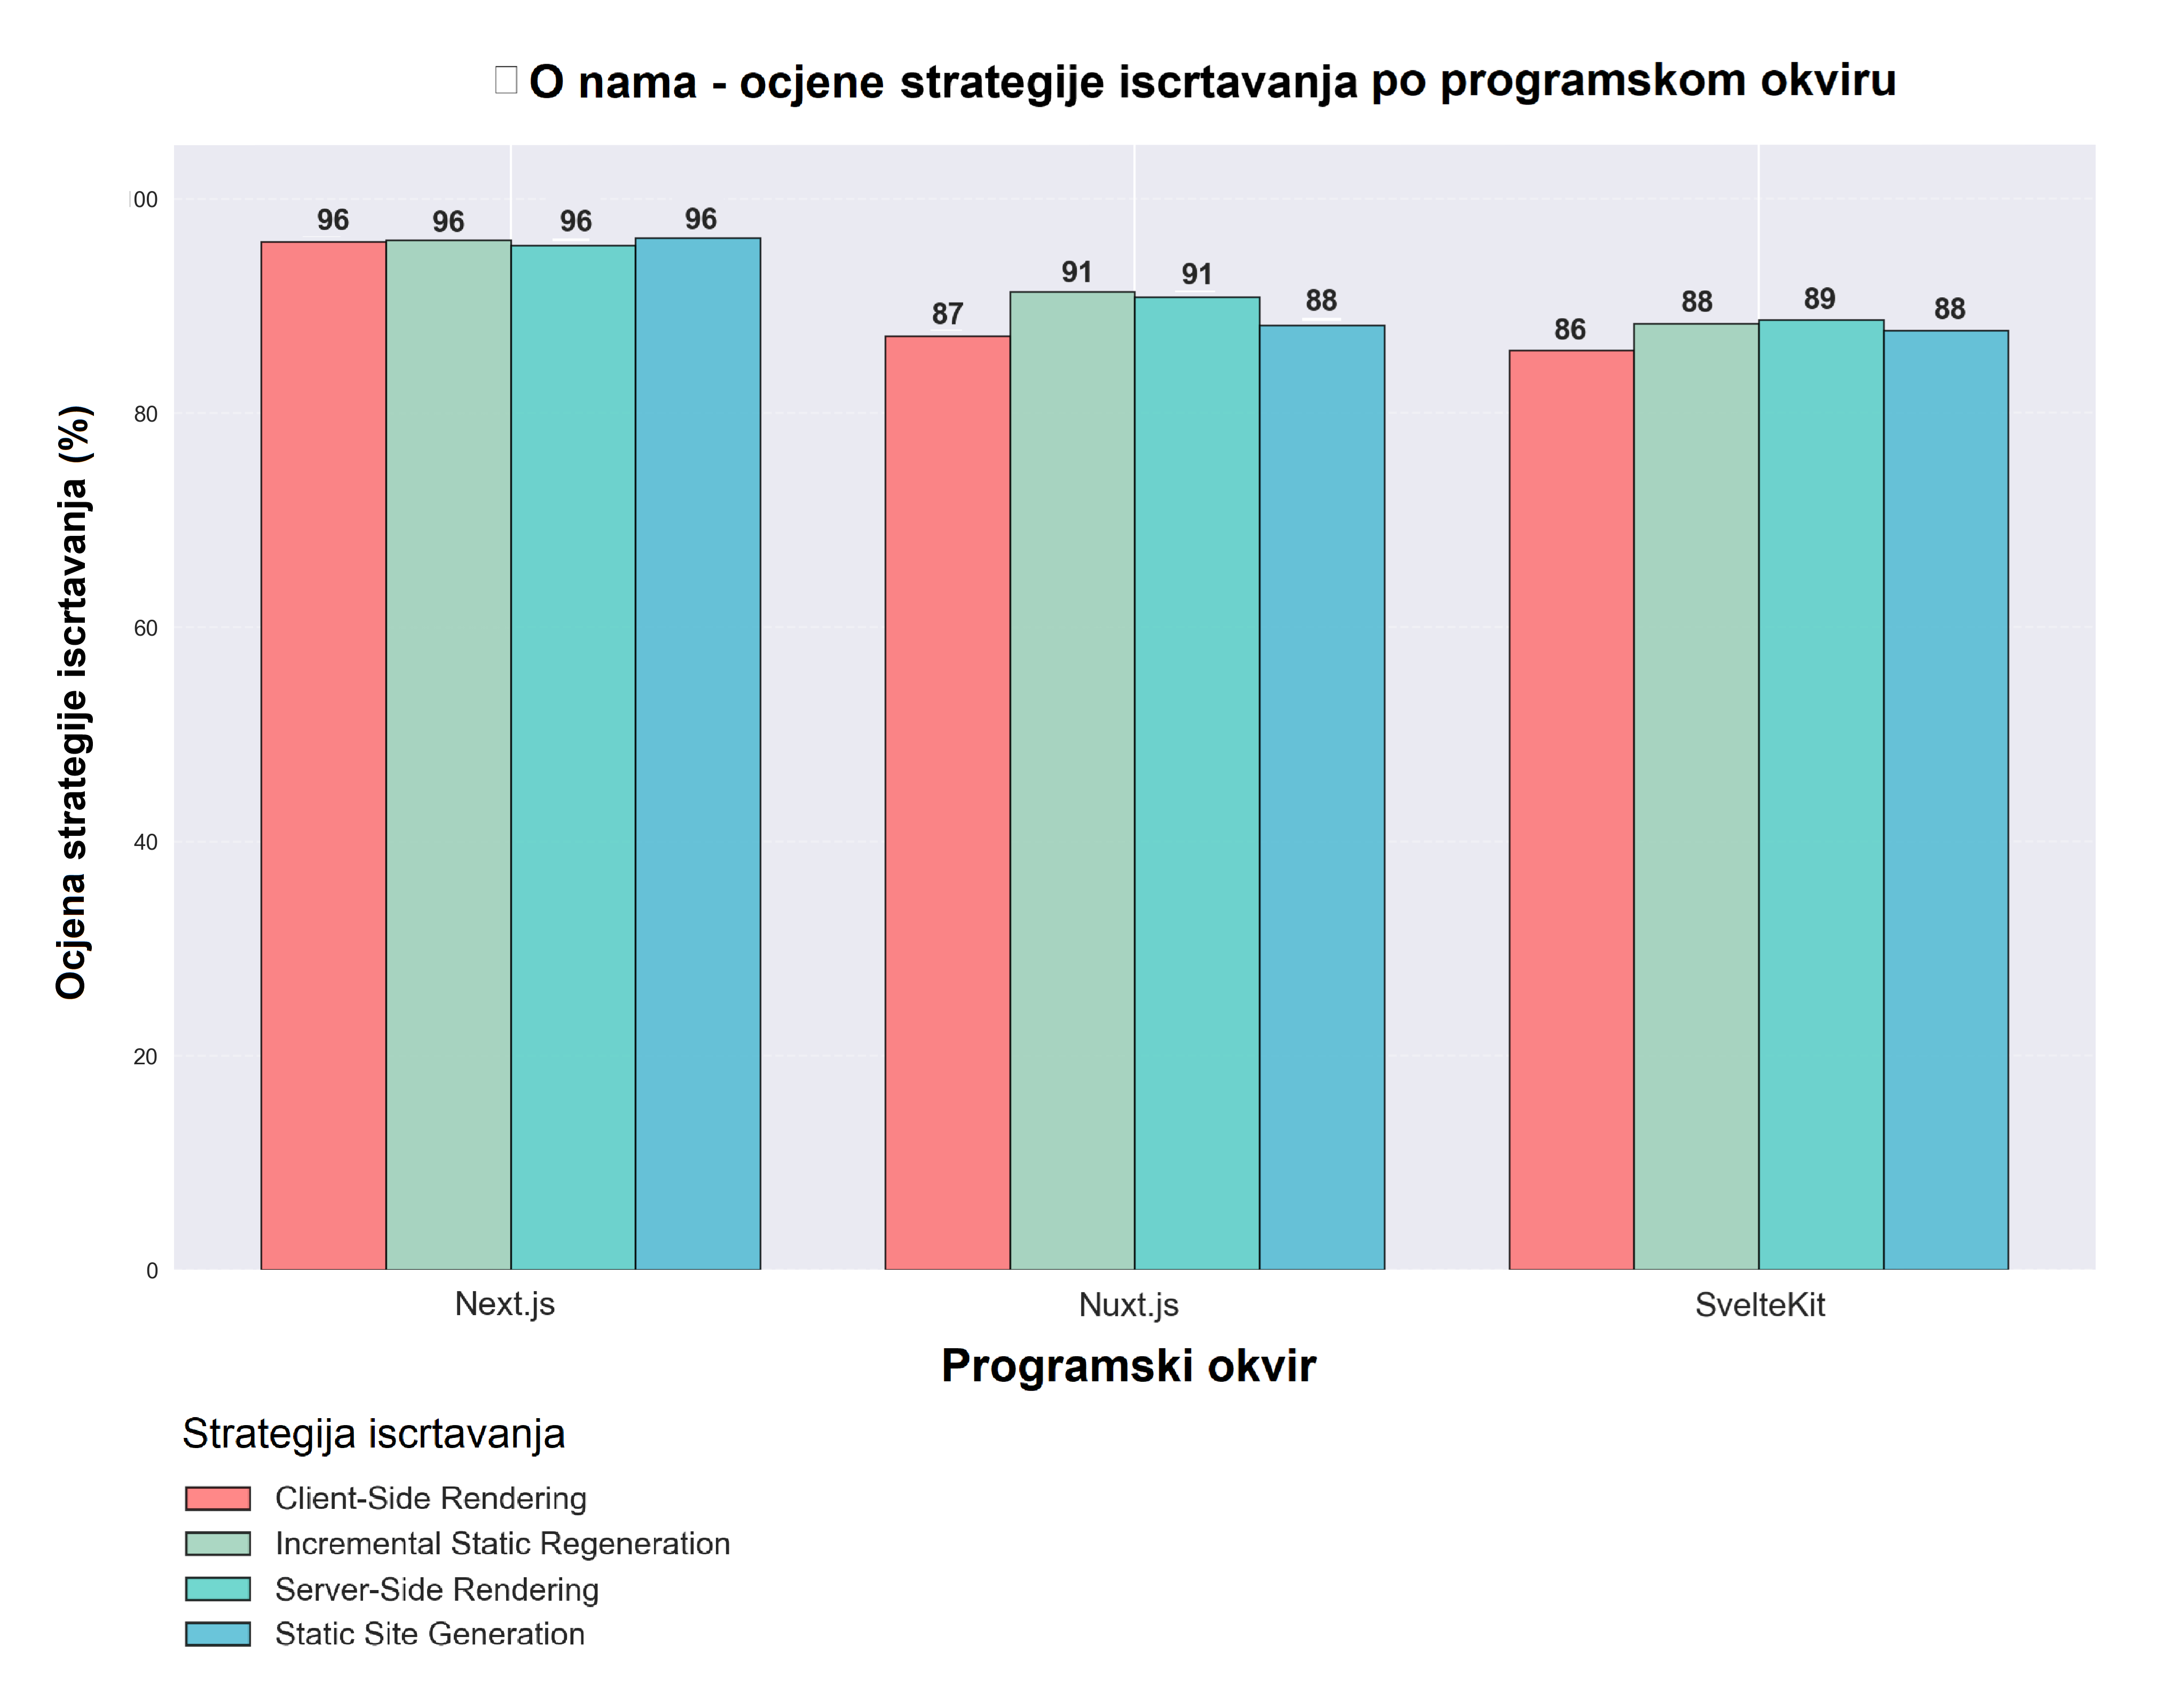
\includegraphics[width=\textwidth]{slike/rezultati/about/about_strategy_comparison.png}
    \caption{Ocjene radnih značajki - usporedba strategija (stranica O nama)}
    \label{fig:testiranje-o-nama-usporedba-strategija}
\end{figure}

\newpage

\subsection{Sažetak rezultata - stranica O nama}

\begin{table}[H]
\centering
\label{tab:sazetak-rezultata-o-nama}
\renewcommand{\arraystretch}{1.5}
\resizebox{\textwidth}{!}{%
    \begin{tabular}{|l|l|l|}
        \hline
        \textbf{Kategorija} & \textbf{Element}                             & \textbf{Ocjena}   \\
        \hline
        \multirow{3}{*}{\textbf{Programski okviri}}
                            & 1. Next.js                                   & 96.0\% (±7.0\%)   \\[0.2em]
                            & 2. Nuxt.js                                   & 89.4\% (±13.2\%)  \\[0.2em]
                            & 3. SvelteKit                                 & 87.6\% (±13.5\%)  \\
        \hline
        \multirow{4}{*}{\textbf{Strategije iscrtavanja}}
                            & 1. Incremental Static Regeneration           & 91.9\% (±11.7\%)  \\[0.2em]
                            & 2. Server-Side Rendering                     & 91.7\% (±11.5\%)  \\[0.2em]
                            & 3. Static Site Generation                    & 90.7\% (±13.0\%)  \\[0.2em]
                            & 4. Client-Side Rendering                     & 89.7\% (±13.0\%)  \\
        \hline
        \multirow{5}{*}{\textbf{Najbolje kombinacije}}
                            & 1. Next.js + Static Site Generation          & 96.3\% (±7.6\%)   \\[0.2em]
                            & 2. Next.js + Incremental Static Regeneration & 96.2\% (±7.1\%)   \\[0.2em]
                            & 3. Next.js + Client-Side Rendering           & 96.0\% (±8.0\%)   \\[0.2em]
                            & 4. Next.js + Server-Side Rendering           & 95.7\% (±7.4\%)   \\[0.2em]
                            & 5. Nuxt.js + Incremental Static Regeneration & 91.3\% (±12.7\%)  \\
        \hline
        \multirow{6}{*}{\textbf{Vodeći po metrici}}
                            & FCP: Next.js + Client-Side Rendering         & 100.0\% (0.920s)  \\[0.2em]
                            & LCP: Nuxt.js + Client-Side Rendering         & 88.0\% (2.590s)   \\[0.2em]
                            & SI: Next.js + Client-Side Rendering          & 100.0\% (1.330s)  \\[0.2em]
                            & TTI: Nuxt.js + Client-Side Rendering         & 98.0\% (2.590s)   \\[0.2em]
                            & TBT: Next.js + Client-Side Rendering         & 100.0\% (8.200ms) \\[0.2em]
                            & CLS: Next.js + Client-Side Rendering         & 100.0\% (0.000)   \\
        \hline
    \end{tabular}%
}
\caption{Sažetak rezultata testiranja stranice O nama}

\end{table}


